%%
%%
%%      SECTION: SENSITIVITY
%%

%% \begin{figure}[htpb]
%% \begin{center}
%% %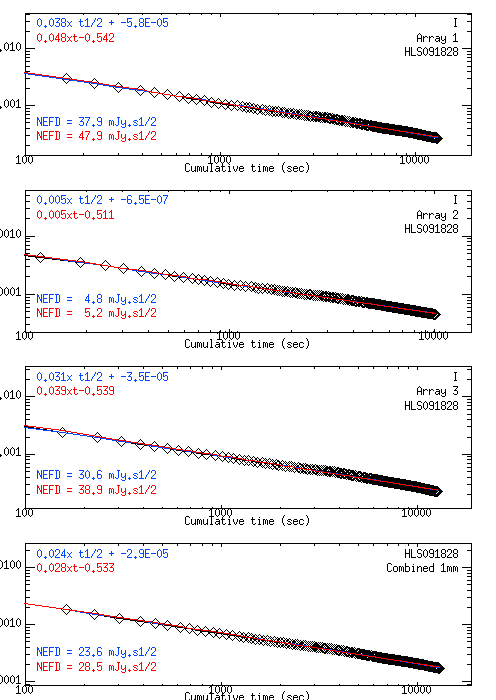
\includegraphics[clip, angle=0, scale =
%% %  0.5]{Figures/NEFD_HLS091828_20170226s415_FXDC0C1_GaussPhot.png}
%% %\includegraphics[clip, angle=0, scale = 0.5]{Figures/nefd_mpfit_HLS091828.eps}
%% \includegraphics[clip, angle=0, scale = 0.4]{Figures/HLS_fit.eps}
%% \includegraphics[clip, angle=0, scale = 0.4]{Figures/HLS_residuals.eps}
%% \caption{Sensitivity on \hls\ vs time of integration. Two power laws are fit:
%%   one with fixed slope $t^{1/2}$ that provides the estimate of the NEFD, one
%%   with a free slope $t^\beta$ to monitor the departure of noise integration from
%%   the canonical $t^{1/2}$. These data come from the integration on \hls\ during
%%   Run9. The difference between the 1 and 2~mm integration time comes from the
%%   density of KIDs in the FOV.}
%% \label{fig:nefd_vs_t}
%% \end{center}
%% \end{figure}

%% {\bf The specs/goals ``NEFD on X \% of pixels'' should be understood as : we have
%% XX\% valid pixels, and with these pixels, we have an NEFD of YY. We should not
%% discard some fraction of our pixels and estimate an NEFD on this subset.}\\

\section{Methodology {\color{blue} Nico}}

The MoU defines the NEFD:  \emph{The Noise Equivalent Flux Density (NEFD)
  is the $1\,\sigma$ sensitivity in one second of effective on-source telescope
  integration time after the absolute calibration has been performed (i.e. after
  beam efficiency and opacity corrections). It is appropriate for 2 mm of
  precipitable water vapor (pwv) content in the atmosphere and 60 degrees
  elevation source. It refers to the inverse variance of the noise on the flux
  measurement of a point-source, averaged over the valid receiver pixels}.

IRAM has its own time estimator for astronomers that will compute the ``effective NEFD'',
provided we give the ``detector NEFD'' and a fraction of valid KIDs $\eta$. To
derive the detector NEFD, we must clearly defined the ``detector time of
integration'' and relate it to the ``time of observation'' which is the time
actually spent by an astronomer at the observing desk. Going from the intuitive
understanding of the time of integration to its actual value is not as trivial
as it seems because of the dependence on the scanning strategy and the
distribution of valid KIDs accross the FOV. We here propose three definitions
with their own merits.

\subsection{Estimating the time of integration}

\subsubsection{Time of integration from the density of samples}

Let's take a map of resolution $r$ (arcsec) and consider the map pixel that is
centered on the position where we estimate the flux uncertainty
$\sigma_\phi$. The number of hits in this pixel $N_h(r)$ allows us to define a
time of integration on this pixel via the sampling frequency $\nu$

\begin{equation}
t_{pix} = N_h(r)/\nu
\end{equation}

To estimate how much wall clock time was necessary to the entire matrix to
produce this density of samples, we need to account for how many KIDs, on
average, contribute to $N_h(r)$ at the same time, that is to say the average
number of KIDs per map pixel. Indeed, if the pixel is large enough to contain
$n$ KIDs at each time, the number of samples in this pixel will be $n$ times
larger for the same time of observation. The same is true if we combine A1 and
A3 for instance. We therefore note $S$ the surface of the FOV, $g$ the distance
between adjacent KIDs and note that $S = N_{pix} \times r^2 = N_{kids} \times
g^2$. The number of KIDs per pixel of $r$\,arcsec resolution is thus $r^2/g^2$,
so the actual observation time reads

\begin{equation}
t_{det} = t_{pix}\frac{g^2}{r^2} = \frac{N_h(r)}{\nu}\frac{g^2}{r^2}
\end{equation}

For the combination of arrays 1 and 3, the number of KIDs per pixel is the sum
of the two contributions that impact the number of KIDs per pixel:

\begin{equation}
t_{det}^{1mm} = \frac{1}{2}\frac{N^{1mm}_h(r)}{\nu}\frac{g^2}{r^2}
\end{equation}

So finally, if $\sigma$ is the uncertainty on the flux estimate, the detector NEFD reads

\begin{equation}
NEFD_{det} = \sigma_\phi\sqrt{t_{det}}
\label{eq:nefd_t_int}
\end{equation}

To relate it to the effective ``observer'' NEFD, we must account for the
fraction of valid pixels actually used to derive the map. Indeed, the
integration time per pixel goes like $\eta$ for the same observation, thus:

\begin{equation}
NEFD_{det}^{eff} = \sigma_\phi\sqrt{t_{det}/\eta}
\end{equation}

which in turn translates into a time requirement to reach the same level of integration:

\begin{equation}
t_{det}^{req} = \left(\frac{NEFD_{det}}{\sigma_\phi}\right)^2\frac{1}{\eta}
\label{eq:t_astro}
\end{equation}

\subsubsection{Time of integration from the matrix footprint}

One can also think of the ``time spent on the source'', for a full matrix
(ie. all valid KIDs), as the time when the source is inside the circular
footprint of the matrix. During a scan, it's easy to count how much time the
source is at a distance from the FOV center that is smaller than the FOV
radius. This time, $t_{geom}$ is a direct estimate of the time ``at the desk'',
so it enters the definition of effective NEFD, not the detector NEFD, hence:

\begin{equation}
NEFD^{eff}_{geom} = \sigma_\phi \sqrt{t_{geom}}
\end{equation}

Fig.~\ref{fig:time_comparison} compares $\eta t_{geom}$ to $t_{det}$ and shows
the good agreement between the two. {\bf Because the definition of $t_{det}$ is more
straightforward in terms of measurement from the map and design parameters and
does not require an approximate determination of the FOV radius, it is our
reference time estimator.}

% \begin{figure}
% \begin{center}
% \includegraphics[clip, angle=0, scale =0.8]{Figures/time_of_integration_0.eps}
% \caption[Time of integration]{Comparison between two estimators of the time of
%   integration on \hls\ during Run~9 for FOV diameter of 6.2~arcmin. The
%   difference goes from 2\% to 5\%, hence translating into a NEFD relative difference of 1
% to 2.5\%.}
% \label{fig:time_comparison}
% \end{center}
% \end{figure}

%% \subsubsection{Time of integration from the flux estimator}
%% 
%% The estimation of the flux of a point source, and its associated uncertainty is
%% done by fitting the amplitude of a gaussian profile of fixed FWHM. In the case
%% of white noise, the flux estimator reads
%% 
%% \begin{equation}
%% \hat{\phi} = \frac{1}{\sum_p g_p^2}\sum_p g_p m_p\,,
%% \label{eq:phi_def}
%% \end{equation}
%% 
%% and its variance is
%% 
%% \begin{equation}
%% \sigma_\phi^2 = \left(\frac{1}{\sum_p g_p^2}\right)^2\sum_p g_p^2\sigma_p^2\,.
%% \label{eq:sigma_phi_def}
%% \end{equation}
%% 
%% In the case of white noise and considering the equivalent of the
%% uniform full matrix of the NEFD definition: $\sigma_p = \sigma_1/\sqrt{N_p}$,
%% where $\sigma_1$ is the standard deviation of 1 sample and $N_p$ is the number of
%% hits in pixel $p$. Accounting for the sampling frequency, it reads
%% 
%% \begin{eqnarray}
%% \sigma_\phi^2 &=& \frac{\sigma_1}{\nu}\left(\frac{1}{\sum_p g_p^2}\right)^2\sum_p \frac{g_p^2}{t_p}\,, \nonumber\\
%% &=&\frac{\sigma_1}{\nu}\frac{1}{t_{beam}}\,
%% \label{eq:sigma_phi_def_2}
%% \end{eqnarray}
%% 
%% where $t_{beam}$ is homogeneous to a time and is such that $\sigma_\phi$ goes
%% like $1/\sqrt{t_{beam}}$.


\subsection{NEFD estimation methods}

With the uncertainty on flux measurements as described in \todo{SECTION XXXXXXXXXXX} and
now an esimator of the time of integration, we have everything in hand to derive
the NEFD. We have devised several ways to estimate it at the same time as
checking the good behaviour of the instrument. Two methods are based on deep
integrations on a source, one is based on the joint analysis of multiple scans
without combining them:

\begin{enumerate}
\item Deep Integration method 1: the error on the flux of a point source for an
  integration time $t$ is $\sigma = NEFD/\sqrt{t}$. Fitting this obtained
  uncertainty against $\sqrt{t}$ must therefore give a straight line whose
  amplitude is the NEFD if correctly corrected for the different elevation and
  opacity conditions of observations.
\item Deep Integration method 2: by summing an large and even number of scans
  with alternative positive and negative weights, we cancel the signal while
  keeping the noise properties. The final ``Jackknife'' map can then be analyzed
  to provide estimates of flux uncertainties for a the effective time of
  integration, hence giving an alternate estimation of the NEFD.
\item Joint analysis method: analyzing each scan in terms of sensitivity and
  time of integration, we have an NEFD per scan that varies with opacity and
  elevation. Fitting the distribution of measures against $e^\tau/sin\delta$
  must provide the zenith opacity.
\end{enumerate}

In this section, we use data of Runs 9 and 12 \todo{XXXXX TBC} on \hls\ and G2.

\hls\ \cite{hls_combes} is moderately faint source, expected to be 74.5\,mJy at
1mm and 15.7\,mJy at 2mm (M.~Bethermin, private communication). This source was
chosen for its flux and its availability during Run9 for long integration. It
has been observed for about 9\,h in total over three nights. The scans were
8x5~arcmin$^2$, alternatively oriented in (ra,dec), (dec,ra), (az,el),
(el,az).

G2 has become the nickname of an empty target close to sources known to IRAM but
not to the commissionning team in order to check our source detection capacities blindly.

The data were processed according to \todo{(cf.~\ref{se:cm1blck}XXXXX)}.

\subsubsection{Deep integration method 1: $\sigma = NEFD/\sqrt{t}$}

%%  and the
%% scans have 
%% \hls. The scans have been combined with standard inverse noise weighting. The
%% noise in each map pixel is derived from the rms of the background corrected by
%% the square root of the number of observations per pixel (N1). If the noise was
%% perfectly gaussian, the distribution of the map signal over this noise estimate
%% (far from the source) would be a normalized gaussian. In practice, this leads to
%% gaussians that 1.6 and 1.5 larger. We therefore increase our noise estimate (N1)
%% by these factors to derive our final estimates. Should the extra sources that
%% pop up in the field contribute to this estimate, they would only make our
%% estimate more conservative.

We co-add the scans one by one and each time perform a photometric analysis on
the map according to {\todo{REF TO SECTION ON PHOTOMETRY}}. The uncertainty on
the flux at the center of the field (on source in the case of \hls, off source
in the case of G2) is plotted and fitted against $sqrt{t_det}$. It should go
like a straight line if scans were all taken in the exact same conditions and
stacked with equal weights. In pratice, the weights are sensitive to the
conditions of observations, namely the elevation and opacities \todo{XXXXX
  (Fig.~\ref{fig:obs_conditions}) XXXX} and they must be accounted for. The
uncertainty on the central flux reads

\begin{equation}
\sigma = NEFD_{det}\times e^{\tau/\sin\delta}\times\sqrt{t}
\label{eq:sigma_nefd}
\end{equation}

Because scans are coadded with inverse variance weighting, the combined flux is

\begin{equation}
\phi = \frac{1}{\sum_n 1/\sigma_n^2}\sum_n\frac{\phi_n}{\sigma_n^2}
\end{equation}

whose variance is

\begin{equation}
\sigma^2 = \frac{1}{\sum_n 1/\sigma_n^2}
\end{equation}

which, according to Eq.~(\ref{eq:sigma_nefd}) becomes

\begin{equation}
\sigma^2 = \frac{NEFD_0^2}{\sum_{n}t_n e^{-2\tau_n/\sin\delta_n}}\,.
\label{eq:sigma_tau_w8}
\end{equation}

If the opacity and the elevations are the same for all scans, we recover the
integration like $\sqrt{t}$. In general, if the observing conditions vary, we
must fit the integrated sensitivity vs the effective time $\sum_{n}t_n
e^{-2\tau_n/\sin\delta_n}$ in order to recover an unbiased estimate of
$NEFD_0$.{\color{red} STOPPED HERE}\\


\subsubsection{Deep integration method 2: Jackknife}

With enough scans of the same soure, it is possible to alternate addition and
subtraction of the scans and therefore cancel the contribution of the signal to
the final combination, while preserving the noise properties. This method is
often refered to as ``Jackknife'' and is a powerful test for residual
systematics. The Jaccknife maps of \hls\ and G2 are presented on
\todo{XXXXX Fig.\ref{figs:jk_maps} XXXX}. Photometry at their center provides estimates of
  the zenith NEFD of \todo{XXXX}


\begin{table}
\begin{tabular}{|l|l|c|c|}
  \hline
              &        & \hls               & G2\\
\hline
{\it Scatter} & A1     & 51.42  & 52.54 \\
              & A3     & 39.55  & 40.03 \\
              & A1\&A3 & 31.32 & 32.71 \\
              & A2     &  8.10  &  8.76 \\
\hline
{\it Jackknife} & A1     & 54.13  & 54.55 \\
                & A3     & 40.88  & 39.12 \\
                & A1\&A3 & 31.83 & 32.50\\
                & A2     &  8.78  &  9.86 \\
\hline
$t^{-1/2}$  & A1     & 51.28  & 49.15\\
            & A3     & 38.79  & 35.54\\
            & A1\&A3 & 30.77 & 30.24\\
            & A2     &  8.39  &  7.94\\
\hline
\end{tabular}

\end{table}
%% \begin{table}
%% \begin{tabular}{|l|c|c|c|c|c|c|}
%% \hline
%% $NEFD_{det}$ [mJy.s$^{1/2}]$                 & \multicolumn{2}{|c|}{Pluto} & \multicolumn{2}{|c|}{\hls} & \multicolumn{2}{|c|}{G2}\\
%% \hline
%% Deep Integration 1: $\sim 1/\sqrt{t}$     & xx & xx    & xx & xx   & xx & xx\\
%% Deep Integration 2: {\it Jackknife}       & xx & xx    & xx & xx   & xx & xx\\
%% Multi scan analysis vs $e^\tau/sin\delta$ & xx & xx    & xx & xx   & xx & xx\\
%% \hline
%% \end{tabular}
%% \caption{\todo{XXXXX}}
%% \end{table}

%% {\tiny
%% \begin{table}
%% \begin{tabular}{|l|c|c|c|c|c|c|c|c|c|c|c|c|}
%%   \hline
%%   & \multicolumn{4}{|c|}{Scatter} & \multicolumn{4}{|c|}{{\it Jackknife}} & \multicolumn{4}{|c|}{$\sim t^{-1/2}$} \\
%%   \hline
%%   & A1 & A3 & A1\&A3 & A2 & A1 & A3 & A1\&A3 & A2 & A1 & A3 & A1\&A3 & A2\\
%%   \hline
%%   HLS091828 & 51.42 & 39.55 & 31.32 &  8.10 & 54.13 & 40.88 & 31.83 &  8.78 & 51.28 & 38.79 & 30.77 &  8.39\\
%%   \hline
%% \end{tabular}
%% \end{table}
%% }


\newpage




 Luckily enough, we have observations of Pluto in very stable
atmospheric conditions and at quasi constant elevation. This will allow us to
check this formalism against more intuitive and direct definitions. We can also
extract from the scans on \hls those that were under stable opacity conditions
and at high and quasi-constant elevation as a confirmation of our final
estimates. The other regimes will help us derive uncertainties our estimates.\\

\begin{figure}[htpb]
\begin{center}
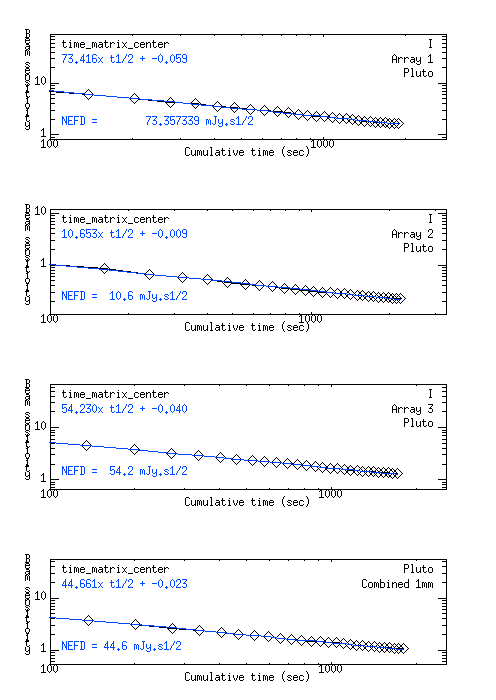
\includegraphics[clip, angle=0, scale=0.4]{Figures/Pluto_8_sigma_vs_time_matrix_center.png}
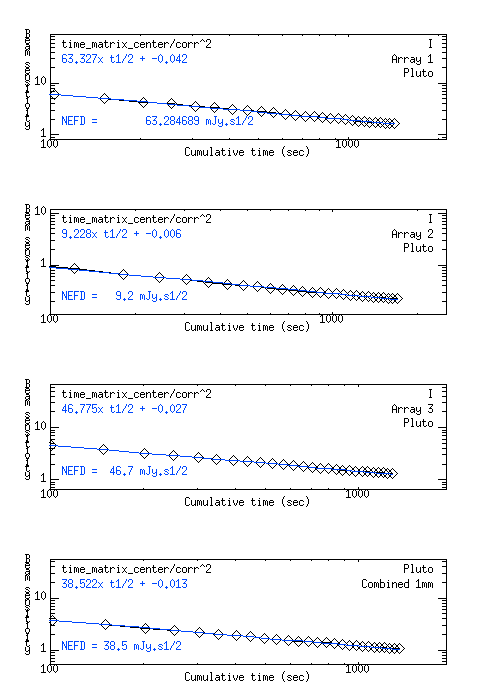
\includegraphics[clip, angle=0, scale=0.4]{Figures/Pluto_8_sigma_vs_time_matrix_center_tau_w8.png}
\caption[Noise decrease with the integration time]{\emph{Left:}$1\,\sigma$ sensitivity vs $t_{int}$ during observations of Pluto, {\bf
  without correction for elevation or opacity}. \emph{Right:} Same fit but this
  time considering the effective time, weighted by opacity and elevation as in Eq.~(\ref{eq:sigma_tau_w8}).}
\label{fig:Pluto_8_sigma_vs_time_matrix_center}
\end{center}
\end{figure}


\begin{figure}[htpb]
\begin{center}
\includegraphics[clip, angle=0, scale=0.4]{Figures/Pluto_5_opacity.eps}
\includegraphics[clip, angle=0, scale=0.4]{Figures/Pluto_5_elevation.eps}
\includegraphics[clip, angle=0, scale=0.4]{Figures/HLS091828_5_opacity.eps}
\includegraphics[clip, angle=0, scale=0.4]{Figures/HLS091828_5_elevation.eps}
\caption[Observing conditions during the noise integration tests]{Opacities and elevations during observations of Pluto and \hls. While
  conditions were stable both in opacity and elevation for Pluto, it was not the
case for \hls.}
\label{fig:pluto_opacities}
\end{center}
\end{figure}

\paragraph{Pluto.} We have 28 scans of Pluto, for a total
integration time of XX at 1mm and XX at
2mm. Fig.~\ref{fig:Pluto_8_sigma_vs_time_matrix_center} shows how the
$1\,\sigma$ sensitivity decreases with $t_{int}$. Considering the small
variations of opacity and elevation during these observations of Pluto
(Fig.~\ref{fig:pluto_opacities}), we can derive an average correction
$exp(-\tau/\sin\delta) = exp(-0.07/\sin(30^\circ)) = 0.87$. This leads to zenith
$NEFD_0^{1mm} = 38.8$ and $NEFD_0^{2mm} = 9.2$\,mJy.s$^{-1/2}$. Using the
jackknife maps and applying the same opacity-elevation correction, one gets
$NEFD_0^{1mm}=38.0$ and $NEFD_0^{2mm}=8.96$.

In light what is discussed in the previous paragraph, if we fit the sensitivity
vs $\sum_{n}t_n e^{-2\tau_n/\sin\delta_n}$, we obtain $NEFD_0^{1mm} = 38.5$ and
$NEFD_0^{2mm}=9.2$. These value are summarized in
tables~\ref{tab:nefd_stable_1mm} and \ref{tab:nefd_stable_2mm}. All these
numbers are obtained with the standard reduction method, a.~k.~a. {\tt
  common\_mode\_one\_block, (CMB)}. If we further subtract a polynomial of order
5 per subscan after this decorrelation (still masking the source), we improve
the results as reported in the tables, while not changing the measured fluxes of
Pluto and HLS (tab.~\ref{tab:fluxes}). We therefore do not change the
calibration with this extra filtering, so the gain in sensitivity does come from
better noise subtraction.

\paragraph{\hls.} While we have an overall
longer integration on \hls, it was acquired during distinct periods, over
varying elevation and different (albeit almost constant by plateau)
opacities (Fig.~\ref{fig:hls_opacities}). Still, performing the same analyses, we obtains the results presented
in tables~\ref{tab:nefd_stable_1mm} and \ref{tab:nefd_stable_2mm}. The values
obtained from the fit vs $1/\sqrt{t}$ are recalled to illustrate the impact of
the opacity-elevation correction on this estimator on \hls\ data. One should
focus on the values derived from the Jackknivfe maps and thoses including the
opacity-elevation correction $1/\sqrt{t_{eff}}$: these values are in very good
agreement when derived from the same reduction method, and in good agreement
between Pluto and \hls.\\

{\bf Conclusion}: while uncertainties on these values should be further
investigated, the good agreement between alternative estimates and at the same
time their differences indicate that they should be valid at about $\pm 1$\,mJy.s$^{1/2}$.
{\bf With these two estimators (fit vs time of integration and
  Jackknife), we find zenith $NEFDs$ below 35 and 9\,mJy.s$^{1/2}$ at 1 and
  2\,mm respectively.} While less intuitive, the more rigourous definition of
the integration time that enters the estimation of the flux, $t_{beam}$, leads to
  slightly different values. It improves by 5\% at 1\,mm, i.e. puts the upper limit at 33.4, but
  degrades the 2\,mm value by the same amount and raise the upper limit to 9.3.

\begin{table}
\begin{tabular}{|l|l|l|l|l|}
\hline
$NEFD_0^{1mm}$~mJy.s$^{1/2}$ & \multicolumn{2}{|c|}{Pluto} & \multicolumn{2}{|c|}{\hls}\\
\hline
Red.~method             & CMB     & CMB+poly5     & CMB & CMB+poly5\\
\hline
$\sim 1/\sqrt{t}$       & 38.8  & 34.3  & 41.7 & 38.2\\
$JK$                    & 35.9  & {\bf 34.7}  & 33.8 & {\bf 33.6} \\
$\sim 1/\sqrt{t_{eff}}$ & 38.5  & {\bf 32.8}  & 37.5 & {\bf 34.4} \\
\hline
\hline
\end{tabular}
\caption[NEFD at 1mm]{Zenith NEFD's in stable elevation and atmospheric conditions on Pluto
  and \hls\ at 1mm.}
\label{tab:nefd_stable_1mm}
\end{table}

\begin{table}
\begin{tabular}{|l|l|l|l|l|}
\hline
$NEFD_0^{2mm}$~mJy.s$^{1/2}$ & \multicolumn{2}{|c|}{Pluto} & \multicolumn{2}{|c|}{\hls}\\
\hline
Red.~method             & CMB     & CMB+poly5     & CMB & CMB+poly5\\
\hline
$\sim 1/\sqrt{t}$       & 9.3 & 8.0 & 9.8  & 8.5\\
$JK$                    & 8.8 & {\bf 7.7} & 8.3  & {\bf 7.6} \\
$\sim 1/\sqrt{t_{eff}}$ & 9.2 & {\bf 8.2} & 9.4  & {\bf 8.2} \\
\hline
\hline
\end{tabular}
\caption[NEFD at 2mm]{Zenith NEFD's in stable elevation and atmospheric conditions on Pluto
  and \hls\ at 2mm.}
\label{tab:nefd_stable_2mm}
\end{table}

\begin{table}
\begin{tabular}{|l|l|l|l|l|}
\hline
Fluxes (mJy) & \multicolumn{2}{|c|}{Pluto} & \multicolumn{2}{|c|}{\hls}\\
\hline
Red.~method  & CMB           & CMB+poly5     & CMB           & CMB+poly5\\
\hline
1\,mm        & $15.0\pm 1.1$ & $13.6\pm 0.9$ & $85.2\pm 0.4$ & $85.4\pm 0.4$\\
2\,mm        & $5.0\pm 0.2$  & $5.0\pm 0.2$  & $14.9\pm 0.1$ & $14.9\pm 0.1$\\
\hline
\hline
\end{tabular}
\caption[Measured fluxes of Pluto and \hls\ with two data reduction methods.]{ The
  extra subtraction of polynomial of order 5 per subscan while masking the
  source does not subtract power to the source, hence the derived sensitivities
  with this methods do not need to be recalibrated.}
\label{tab:fluxes}
\end{table}

%% Tab.~\ref{tab:nefd}. Fig.~\ref{fig:nefd_vs_t} shows the decrease of the
%% uncertainty on the measured flux at the center of the map as a function of
%% time. We either fit a power law or fix the power law to -0.5 and fit only the
%% amplitude. Uncertainties on these values have been estimated via a bootstrap
%% method: we randomize the scans and derive the standard deviation of the average
%% of $n$ scans for any $n$ between 1 and the total number of scans. This gives us
%% an estimate of the uncertainty on $\sigma_\phi$ for a time of integration
%% corresponding to $n$ scans. Strictly speaking, all the scans do not have the
%% exact same duration, but the difference is negligible here.

%% \begin{table}
%% \begin{tabular}{|l|l|l|l|l|}
%% \hline
%% Array & Free power law & Fixed power law $t^{-0.5}$ & Jackknife & Instrument \\
%% \hline
%% A1       & $47.9$ mJy.s$^{-0.54}$ & $37.9$ mJy.s$^{1/2}$ & 35.6 mJy.s$^{1/2}$ & $33.3$ (5) mJy.s$^{1/2}$\\
%% A2       & $5.2$  mJy.s$^{-0.51}$ & $4.8$  mJy.s$^{1/2}$ & 5.7  mJy.s$^{1/2}$ & $5.8$  (5) mJy.s$^{1/2}$\\
%% A3       & $38.9$ mJy.s$^{-0.54}$ & $30.6$ mJy.s$^{1/2}$ & 30.4 mJy.s$^{1/2}$ & $28.4$ (4) mJy.s$^{1/2}$\\
%% A1 \& A3 & $28.5$ mJy.s$^{-0.53}$ & $23.6$ mJy.s$^{1/2}$ & 22.4 mJy.s$^{1/2}$ & $21.1$ (3) mJy.s$^{1/2}$\\
%% \hline
%% \end{tabular}
%% \label{tab:nefd}
%% \caption{Noise integration with observation time and associated derivations of
%%   the NEFD. These values do not account for the extra {\color{red} \bf XXXX \%}
%%   uncertainty on absolute calibration.}
%% \end{table}
%       33.325263       5.2024647
%       28.397230       4.5723151
%       21.143376       4.1538804
%       5.7628233       3.3094792


